cj\subsection{Admin}

\subsubsection{Login}

\textbf{Role:} Admin

\begin{itemize}
    \item \textbf{Function trigger:} The admin enters account credentials and selects the login button.

    \item \textbf{Function description:}
    \begin{itemize}
        \item \textbf{Purpose:}
        \begin{enumerate}
            \item Verify the administrator identity.
            \item Provide access to administrative functions.
        \end{enumerate}

        \item \textbf{Data processing:}
        \begin{enumerate}
            \item The admin enters username and password.
            \item The system validates the credentials.
            \item The system identifies the ADMIN role.
            \item The system creates an admin session.
        \end{enumerate}
    \end{itemize}

    \item \textbf{Function details:}
    \begin{itemize}
        \item Successful login redirects to the Admin Dashboard.
        \item Invalid credentials show an error message.
        \item Admin can access system management screens after login.
    \end{itemize}
\end{itemize}

\textbf{Screen layout:}

\begin{figure}[H]
    \centering
    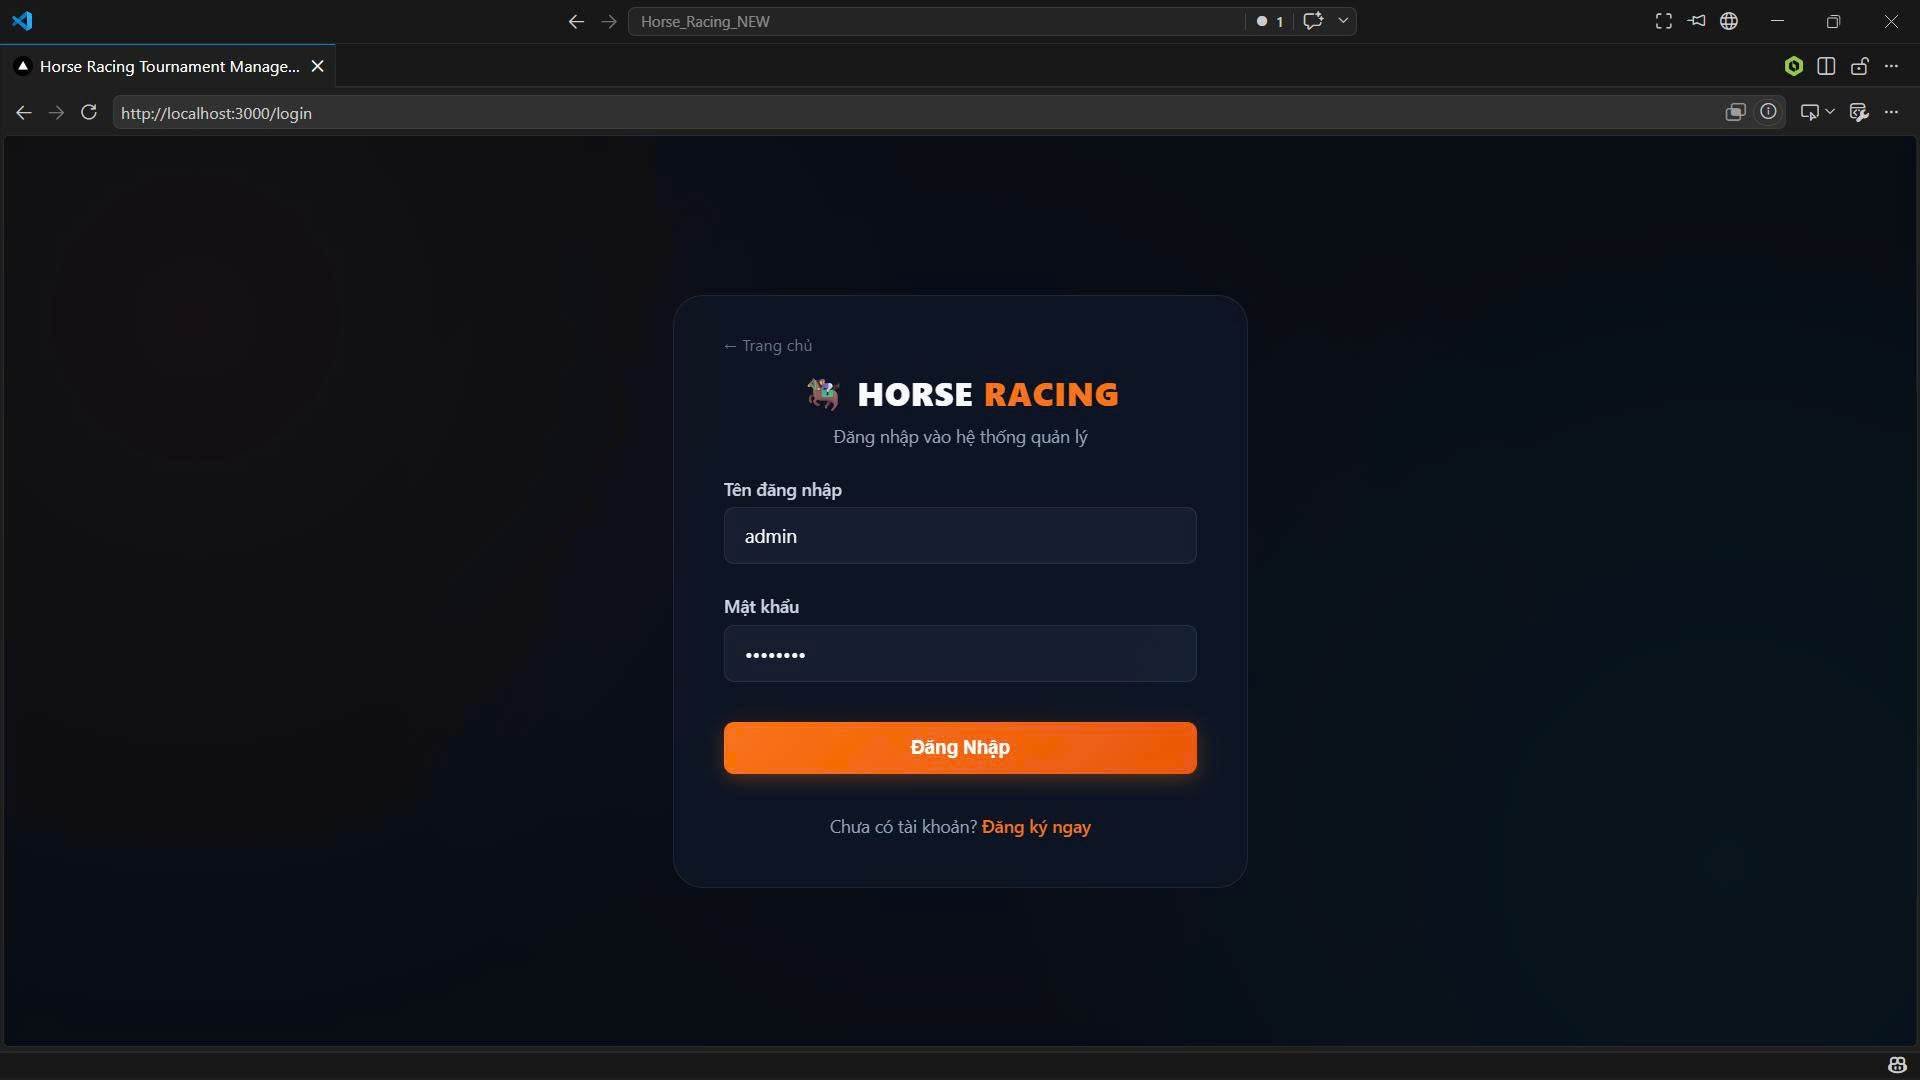
\includegraphics[width=0.7\textwidth]{figures/web_application/admin_img/admin_login.png}
    \caption{Admin Login}
\end{figure}

% ===================================================

\subsection{System Overview}

\textbf{Role:} Admin

\begin{itemize}
    \item \textbf{Function trigger:} Select "Tong quan he thong" from the admin menu.

    \item \textbf{Function description:}
    \begin{itemize}
        \item \textbf{Purpose:}
        \begin{enumerate}
            \item Provide a summary of system status.
            \item Display key metrics and role distributions.
        \end{enumerate}

        \item \textbf{Data processing:}
        \begin{enumerate}
            \item Retrieve user counts by role.
            \item Retrieve tournament and race statistics.
            \item Retrieve award and registration metrics.
        \end{enumerate}
    \end{itemize}

    \item \textbf{Function details:}
    \begin{itemize}
        \item Display total active users, tournaments, races, horses, and awards.
        \item Show distribution of users by role.
        \item Show tournament status and prediction statistics.
    \end{itemize}
\end{itemize}

\textbf{Screen layout:}

\begin{figure}[H]
    \centering
    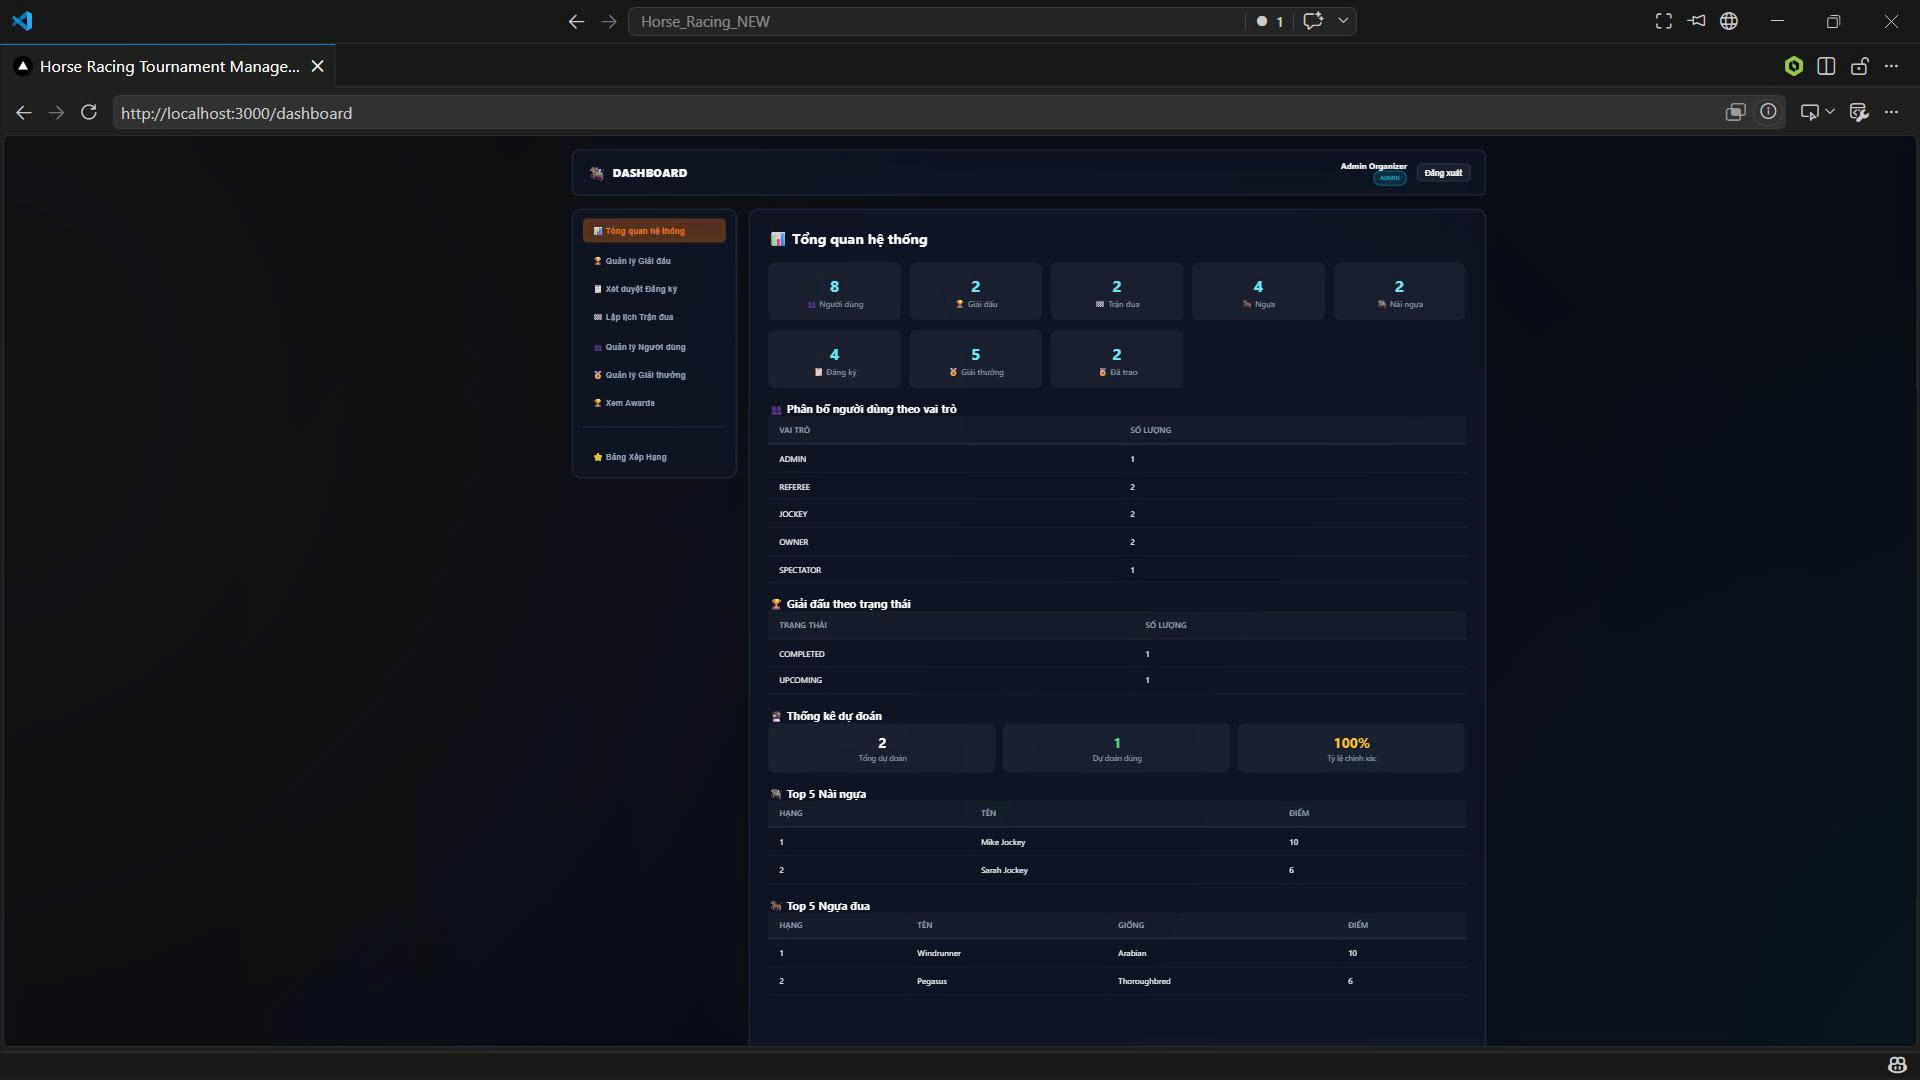
\includegraphics[width=\textwidth]{figures/web_application/admin_img/system_overview.png}
    \caption{System Overview}
\end{figure}

% ===================================================

\subsection{Manage Tournaments}

\textbf{Role:} Admin

\begin{itemize}
    \item \textbf{Function trigger:} Select "Quan ly Giai dau".

    \item \textbf{Function description:}
    \begin{itemize}
        \item \textbf{Purpose:}
        \begin{enumerate}
            \item Create and manage tournament information.
            \item Add new rounds to tournaments.
        \end{enumerate}

        \item \textbf{Data processing:}
        \begin{enumerate}
            \item Enter tournament name, description, dates, and location.
            \item Save tournament details.
            \item Add competition rounds with sequence order.
        \end{enumerate}
    \end{itemize}

    \item \textbf{Function details:}
    \begin{itemize}
        \item Create new tournaments.
        \item Edit or delete tournaments.
        \item Manage the number and order of rounds.
        \item Display current tournament list and status.
    \end{itemize}
\end{itemize}

\textbf{Screen layout:}

\begin{figure}[H]
    \centering
    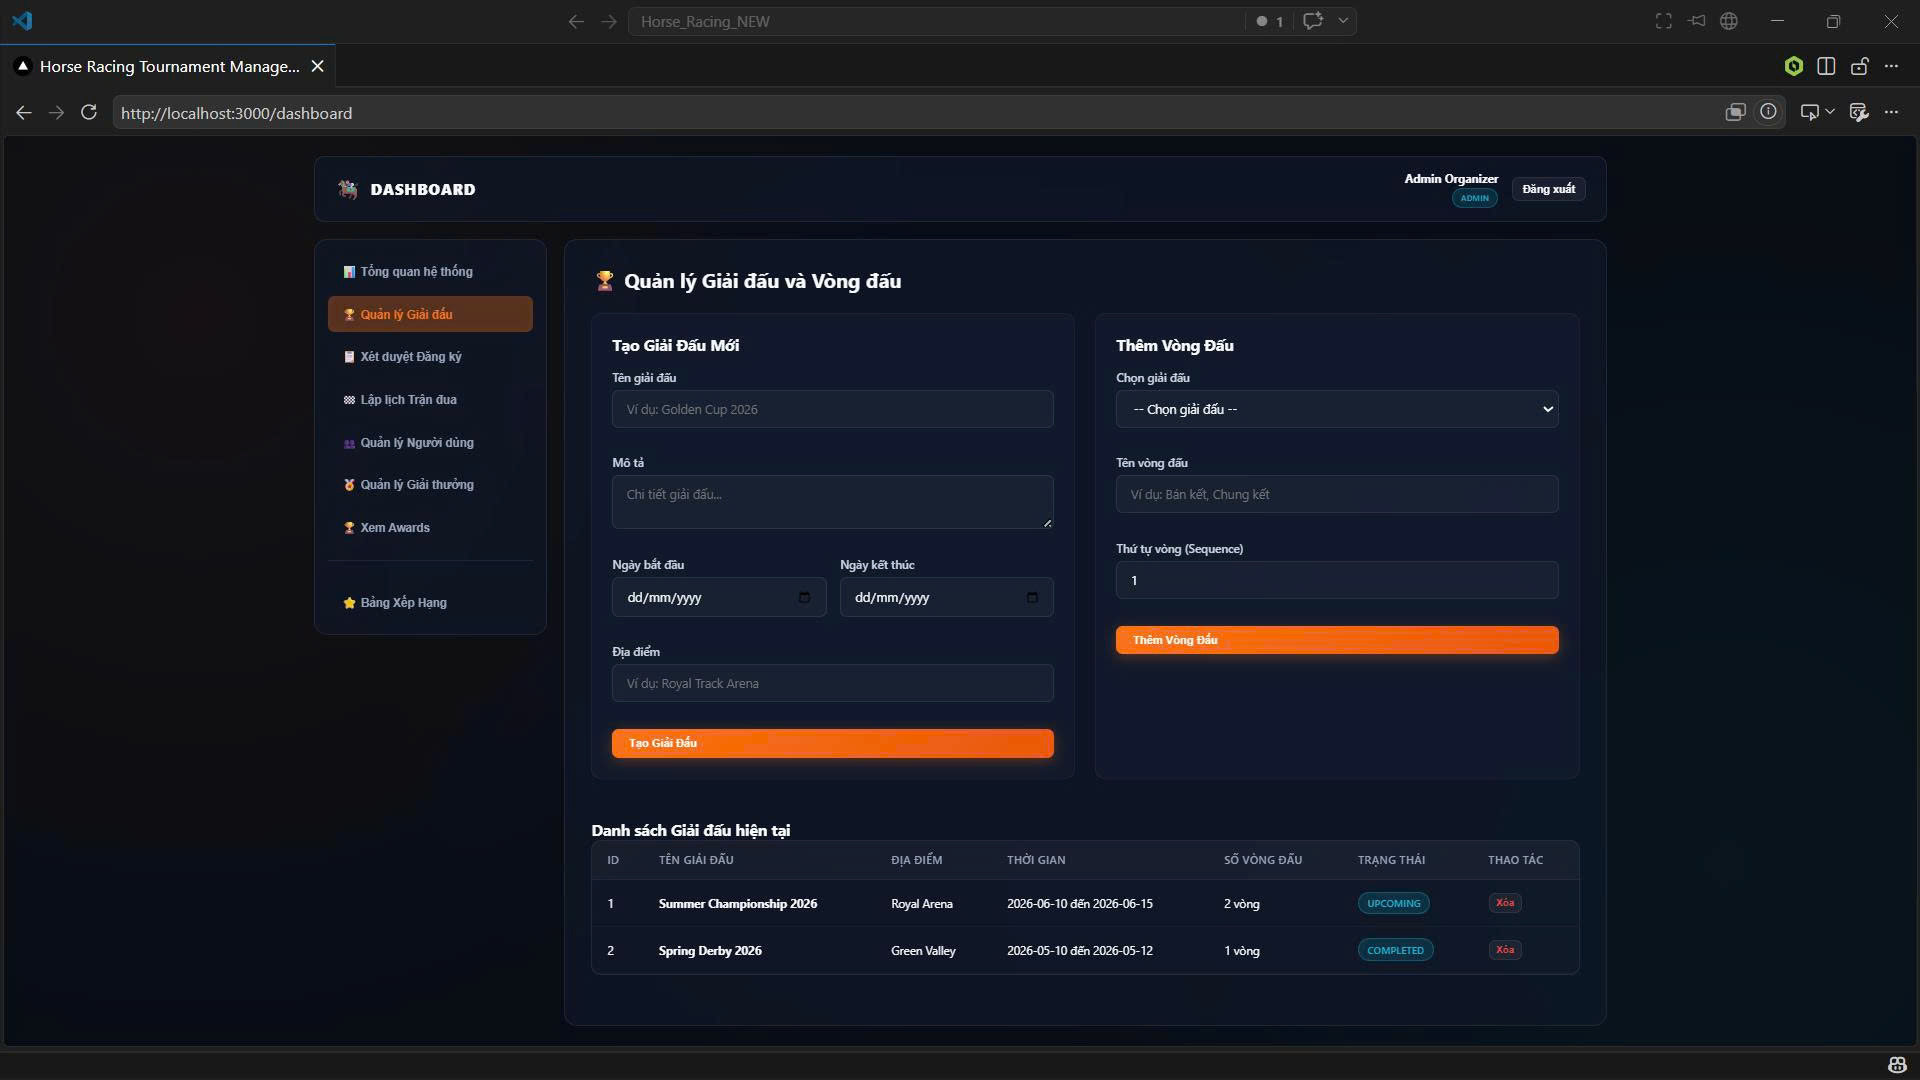
\includegraphics[width=\textwidth]{figures/web_application/admin_img/manage_tournament.png}
    \caption{Manage Tournaments}
\end{figure}

% ===================================================

\subsection{Schedule Races}

\textbf{Role:} Admin

\begin{itemize}
    \item \textbf{Function trigger:} Select "Lap lich Tran dua".

    \item \textbf{Function description:}
    \begin{itemize}
        \item \textbf{Purpose:}
        \begin{enumerate}
            \item Schedule race heats and assign race details.
            \item Organize race lanes and pairs.
        \end{enumerate}

        \item \textbf{Data processing:}
        \begin{enumerate}
            \item Choose the tournament round.
            \item Enter race name, date, distance, and conditions.
            \item Select approved horse-jockey pairs.
            \item Assign lane numbers for each pair.
        \end{enumerate}
    \end{itemize}

    \item \textbf{Function details:}
    \begin{itemize}
        \item Create and manage races.
        \item Assign horses and jockeys to lanes.
        \item Display current race schedule and status.
    \end{itemize}
\end{itemize}

\textbf{Screen layout:}

\begin{figure}[H]
    \centering
    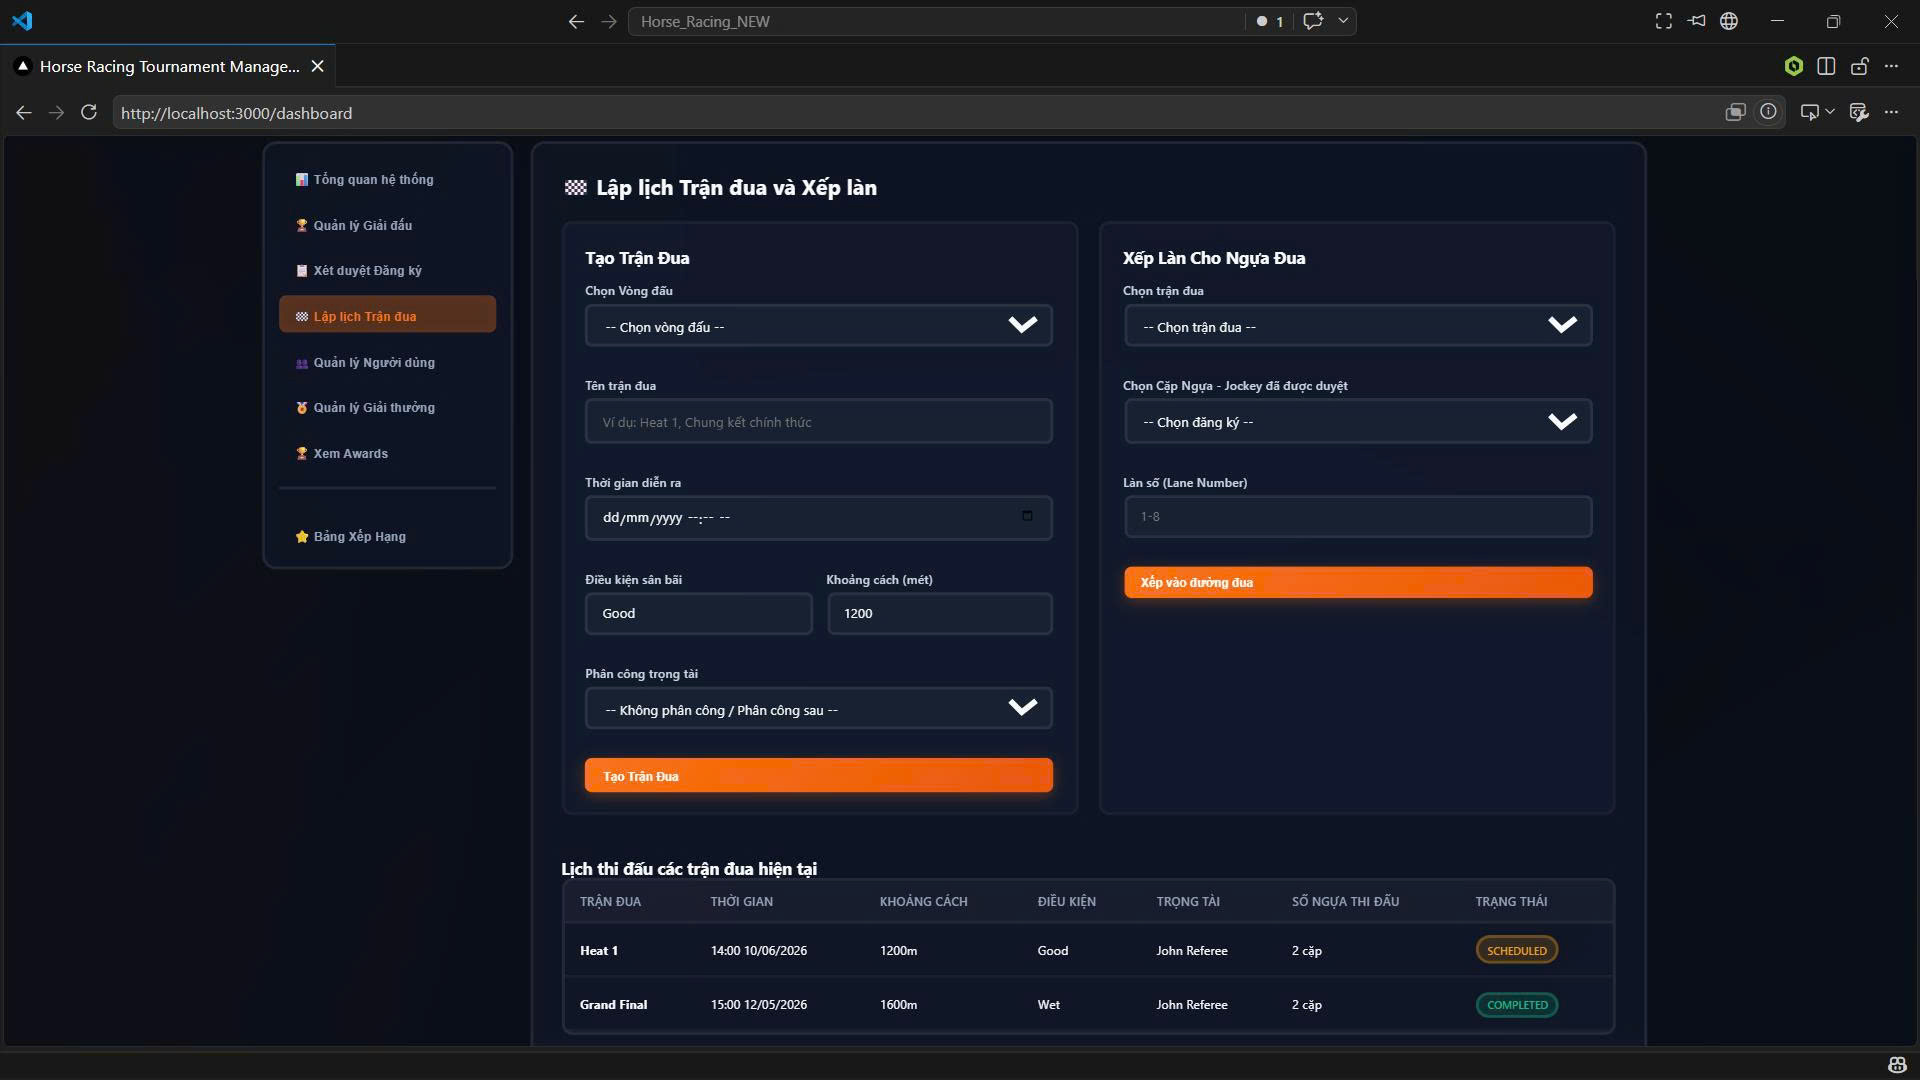
\includegraphics[width=\textwidth]{figures/web_application/admin_img/schedule_race.png}
    \caption{Schedule Races}
\end{figure}

% ===================================================

\subsection{Manage Rewards}

\textbf{Role:} Admin

\begin{itemize}
    \item \textbf{Function trigger:} Select "Quan ly Giai thuong".

    \item \textbf{Function description:}
    \begin{itemize}
        \item \textbf{Purpose:}
        \begin{enumerate}
            \item Define prizes for tournament positions.
            \item Manage award distributions.
        \end{enumerate}

        \item \textbf{Data processing:}
        \begin{enumerate}
            \item Select the tournament.
            \item Enter prize rank, title, value, and description.
            \item Save reward information.
        \end{enumerate}
    \end{itemize}

    \item \textbf{Function details:}
    \begin{itemize}
        \item Add new awards for tournaments.
        \item Edit or delete existing awards.
        \item Display award list and delivery status.
    \end{itemize}
\end{itemize}

\textbf{Screen layout:}

\begin{figure}[H]
    \centering
    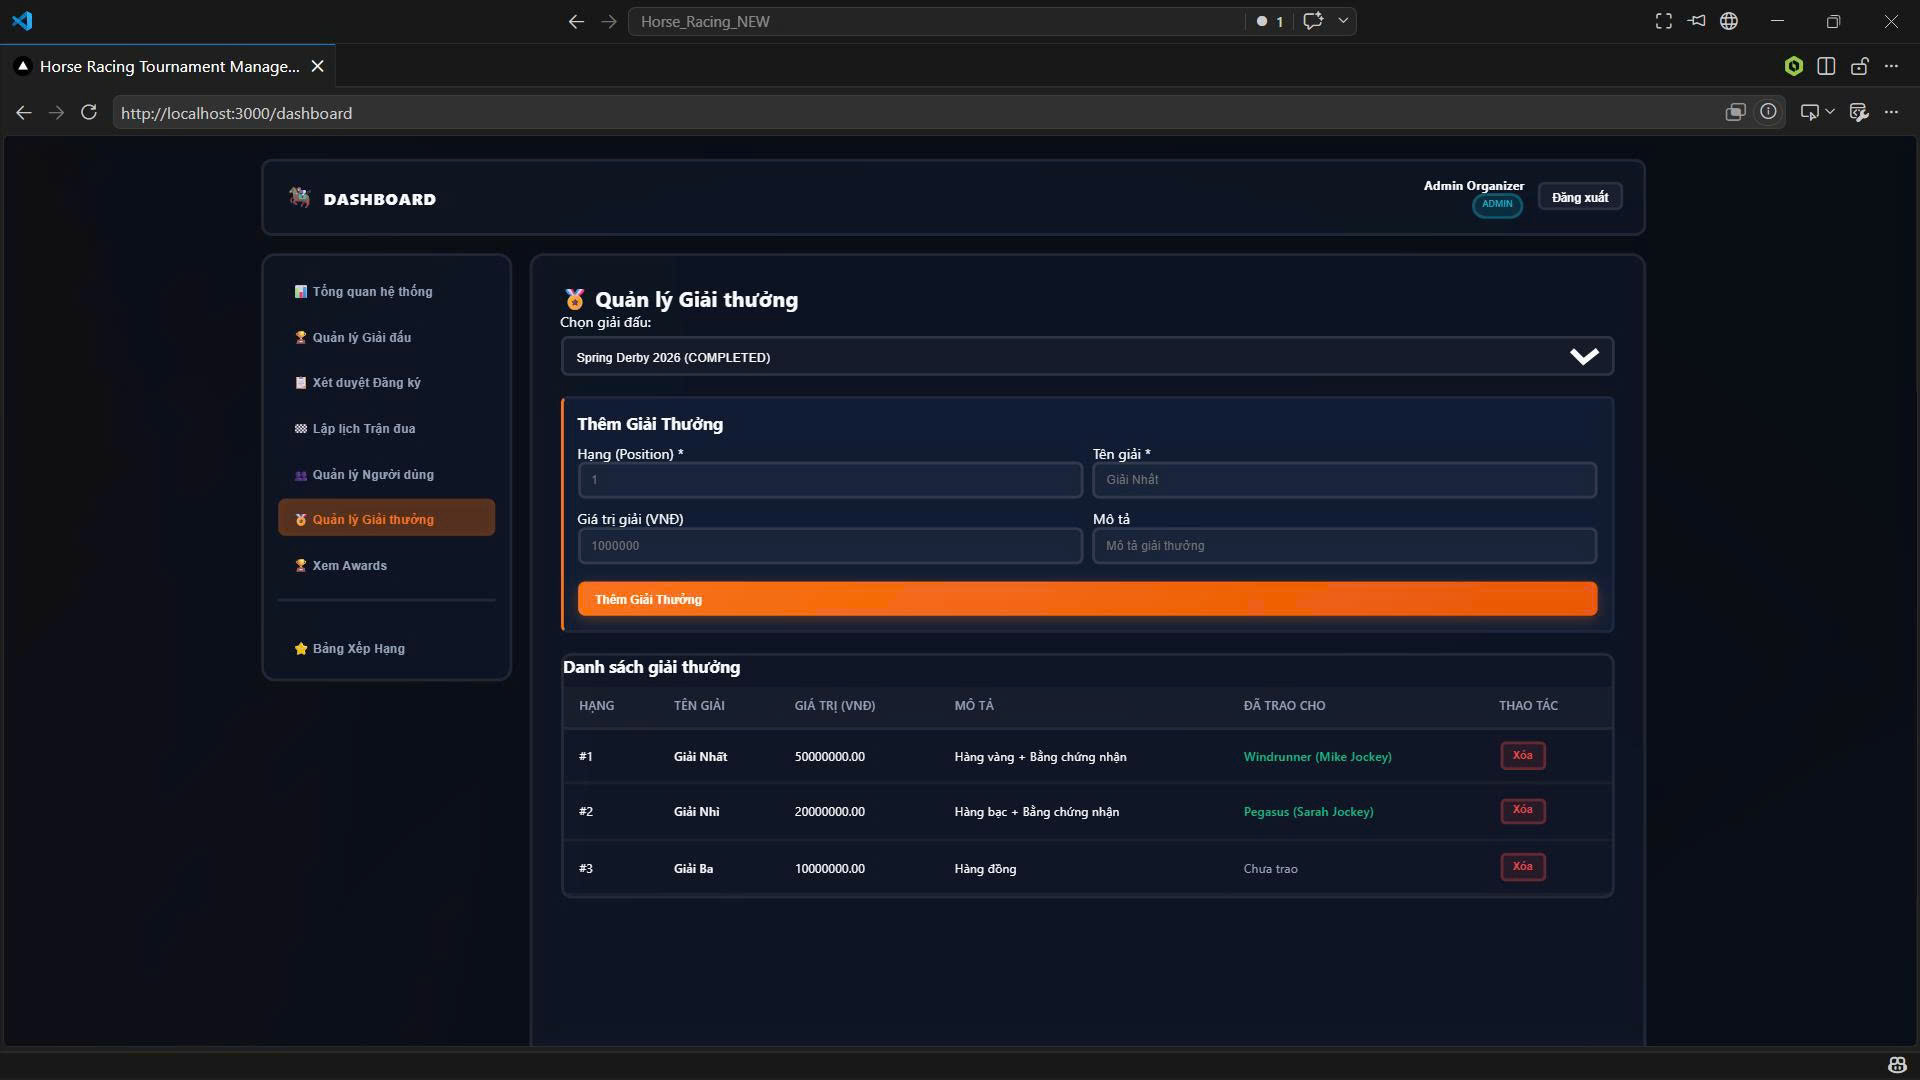
\includegraphics[width=\textwidth]{figures/web_application/admin_img/manage_reward.png}
    \caption{Manage Rewards}
\end{figure}

% ===================================================

\subsection{User Management}

\textbf{Role:} Admin

\begin{itemize}
    \item \textbf{Function trigger:} Select "Quan ly Nguoi dung".

    \item \textbf{Function description:}
    \begin{itemize}
        \item \textbf{Purpose:}
        \begin{enumerate}
            \item Manage system users and roles.
            \item Control access and account status.
        \end{enumerate}

        \item \textbf{Data processing:}
        \begin{enumerate}
            \item Retrieve user accounts.
            \item Display role and status information.
            \item Perform account lock or unlock actions.
        \end{enumerate}
    \end{itemize}

    \item \textbf{Function details:}
    \begin{itemize}
        \item Display user list with roles and statuses.
        \item Lock or unlock user accounts.
        \item Filter users by role.
    \end{itemize}
\end{itemize}

\textbf{Screen layout:}

\begin{figure}[H]
    \centering
    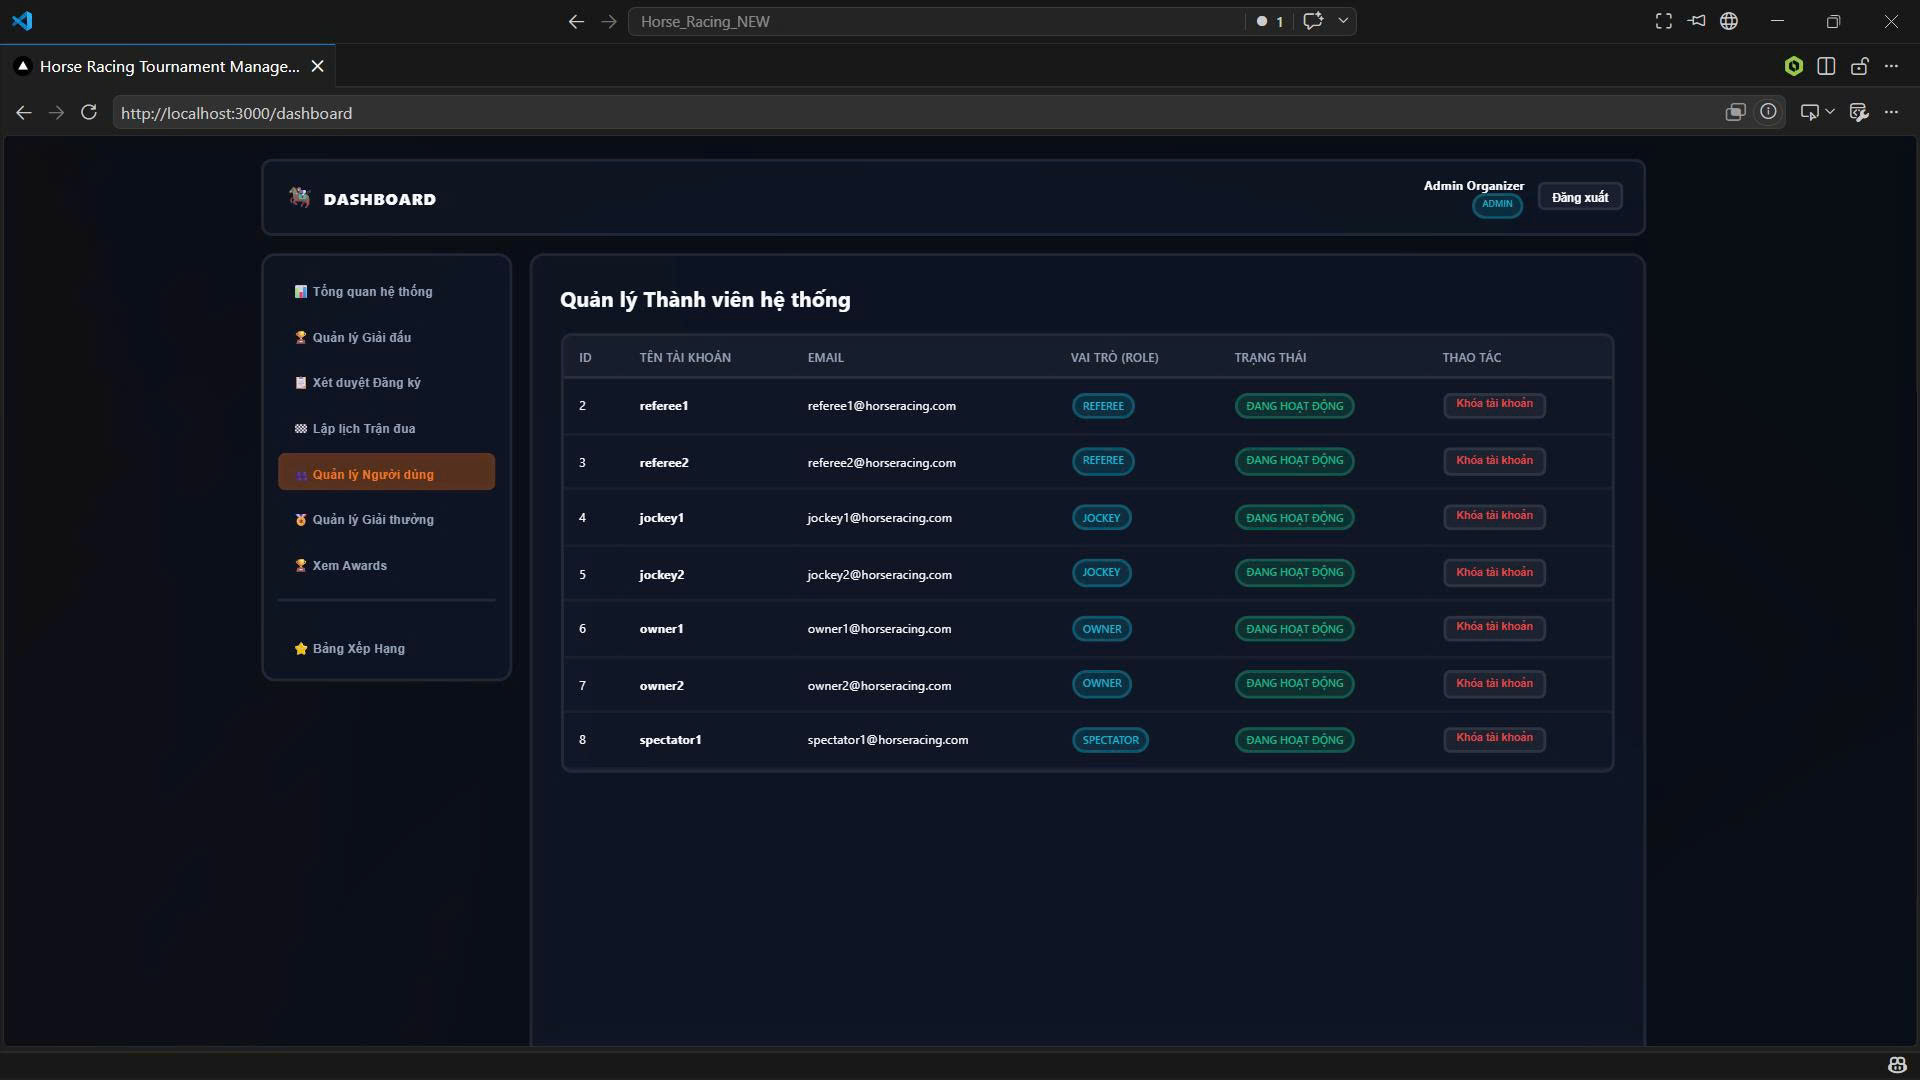
\includegraphics[width=\textwidth]{figures/web_application/admin_img/user_management.png}
    \caption{User Management}
\end{figure}

% ===================================================

\subsection{Confirm Registrations}

\textbf{Role:} Admin

\begin{itemize}
    \item \textbf{Function trigger:} Select "Xet duyet Dang ky".

    \item \textbf{Function description:}
    \begin{itemize}
        \item \textbf{Purpose:}
        \begin{enumerate}
            \item Review and confirm registration requests.
            \item Approve or reject tournament entries.
        \end{enumerate}

        \item \textbf{Data processing:}
        \begin{enumerate}
            \item Retrieve pending registrations.
            \item Display horse, jockey, and tournament details.
            \item Update registration approval status.
        \end{enumerate}
    \end{itemize}

    \item \textbf{Function details:}
    \begin{itemize}
        \item Show pending registration entries.
        \item Approve or reject registrations.
        \item Display current approval status.
    \end{itemize}
\end{itemize}

\textbf{Screen layout:}

\begin{figure}[H]
    \centering
    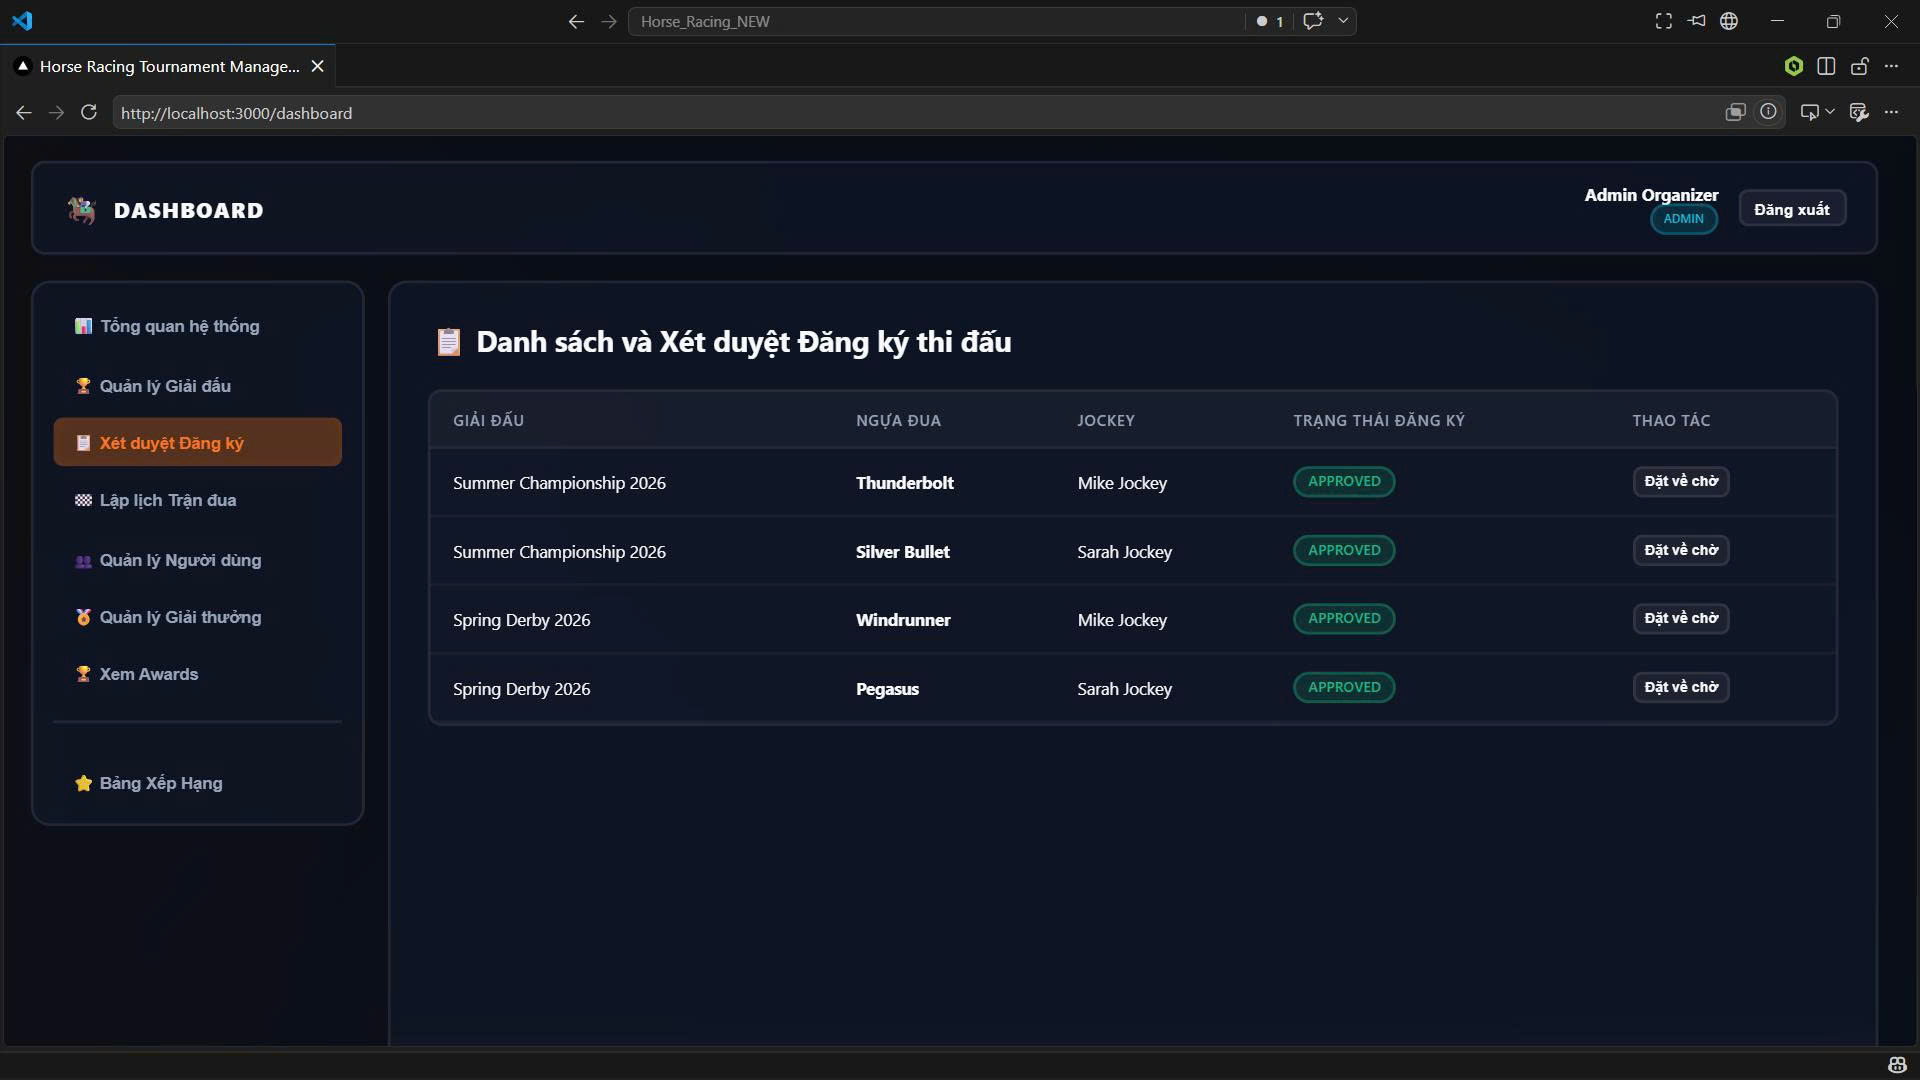
\includegraphics[width=\textwidth]{figures/web_application/admin_img/confirm_register.png}
    \caption{Confirm Registrations}
\end{figure}

% ===================================================

\subsection{Leaderboard}

\textbf{Role:} Admin

\begin{itemize}
    \item \textbf{Function trigger:} Select "Xem Awards" or "Bang Xep Hang".

    \item \textbf{Function description:}
    \begin{itemize}
        \item \textbf{Purpose:}
        \begin{enumerate}
            \item Display the official leaderboard.
            \item Review award winners and rankings.
        \end{enumerate}

        \item \textbf{Data processing:}
        \begin{enumerate}
            \item Retrieve ranking data for horses and jockeys.
            \item Retrieve award recipient details.
        \end{enumerate}
    \end{itemize}

    \item \textbf{Function details:}
    \begin{itemize}
        \item Display award and ranking summaries.
        \item Show top positions by horse and jockey performance.
    \end{itemize}
\end{itemize}

\textbf{Screen layout:}

\begin{figure}[H]
    \centering
    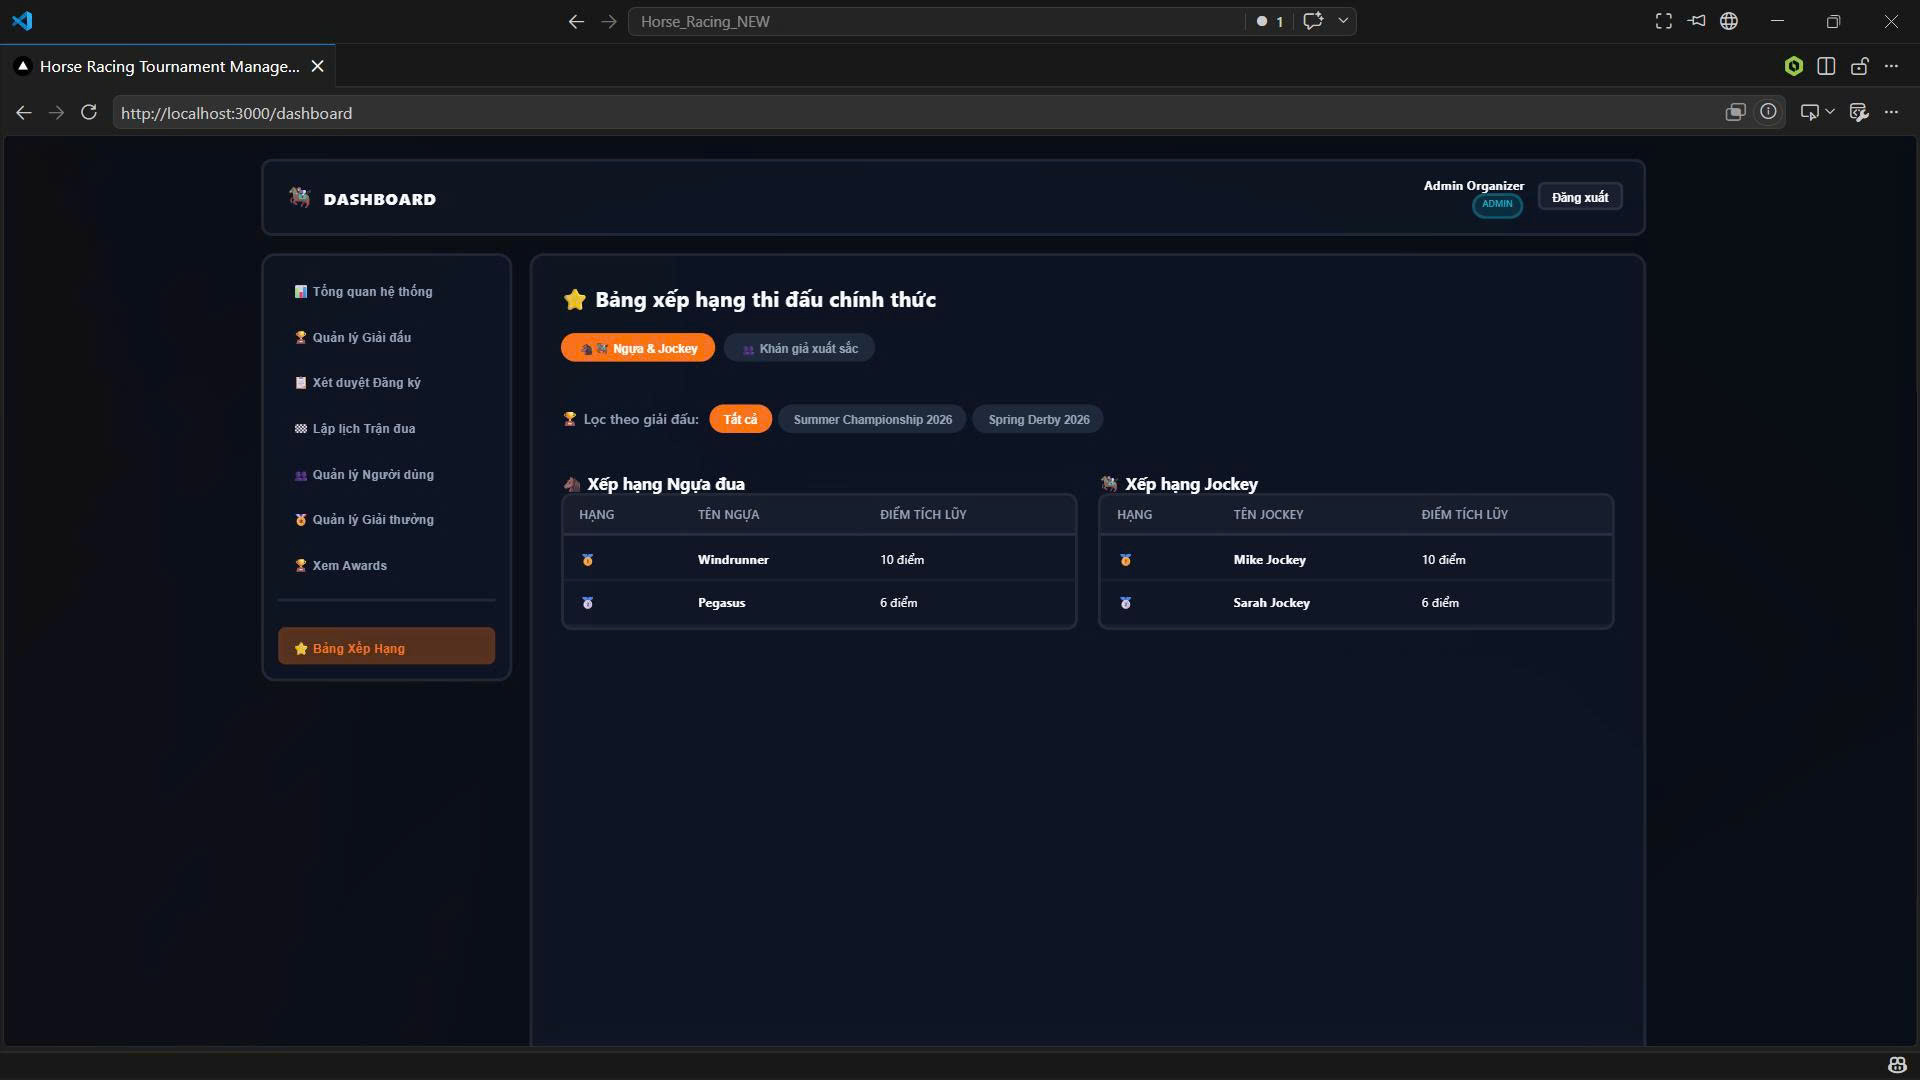
\includegraphics[width=\textwidth]{figures/web_application/admin_img/leaderboard.png}
    \caption{Leaderboard}
\end{figure}
